%%%%%%%%%%%%%%%%%%%%%%%%%%%%%%%%%%%%%%%%%
% Beamer Presentation
% LaTeX Template
% Version 1.0 (10/11/12)
%
% This template has been downloaded from:
% http://www.LaTeXTemplates.com
%
% License:
% CC BY-NC-SA 3.0 (http://creativecommons.org/licenses/by-nc-sa/3.0/)
%
%%%%%%%%%%%%%%%%%%%%%%%%%%%%%%%%%%%%%%%%%

%----------------------------------------------------------------------------------------
% PACKAGES AND THEMES
%----------------------------------------------------------------------------------------

\documentclass[10pt,xcolor={dvipsnames}]{beamer}
%\setbeamersize{text margin left=1em,text margin right=1em}
\usepackage{mathtools}
\usepackage{amsmath}
\usepackage{bm}
\usepackage{hyperref}

\usepackage{graphicx} % Allows including images
\graphicspath{{/Users/rebecca/Documents/Rivet_Analyses/MC_VBFDM/PlotCombinationTool/Figures/}{/Users/rebecca/Documents/Presentations/Talks/}{/Users/rebecca/Documents/Rivet_Analyses/MC_VBFDM/PlotCombinationTool/Figures/StatPlots/}{/Users/rebecca/Documents/Rivet_Analyses/MC_VBFDM/PlotCombinationTool/Figures/2DHists/}{/Users/rebecca/Documents/JER/MinimiseMatrixJER/Difference_PowhegPythia/}{/Users/rebecca/Documents/Presentations/Reports/}}
\usepackage{booktabs} % Allows the use of \toprule, \midrule and \bottomrule in tables

\usepackage{etoolbox}
\usepackage{cancel}

\usepackage{subcaption}
\captionsetup{compatibility=false}

\usepackage{multirow}

\usepackage{appendixnumberbeamer}

%\newlength\origleftmargini
%\setlength\origleftmargini\leftmargini
%\setbeamertemplate{itemize/enumerate body begin}{\setlength{\leftmargini}{2pt}}%

%\let\oldexampleblock\exampleblock
%\let\oldendexampleblock\endexampleblock
%\def\exampleblock{\begingroup \setbeamertemplate{itemize/enumerate body begin}{\setlength{\leftmargini}{\origleftmargini}} \oldexampleblock}
%\def\endexampleblock{\oldendexampleblock \endgroup}%

%\let\oldalertblock\alertblock
%\let\oldendalertblock\endalertblock
%\def\alertblock{\begingroup \setbeamertemplate{itemize/enumerate body begin}{\setlength{\leftmargini}{\origleftmargini}} \oldalertblock}
%\def\endalertblock{\oldendalertblock \endgroup}

\mode<presentation> {

% The Beamer class comes with a number of default slide themes
% which change the colors and layouts of slides. Below this is a list
% of all the themes, uncomment each in turn to see what they look like.

%\usetheme{default}
%\usetheme{AnnArbor}
%\usetheme{Antibes}
%\usetheme{Bergen}
%\usetheme{Berkeley}
%\usetheme{Berlin}
\usetheme{Boadilla}
%\usetheme{CambridgeUS}
%\usetheme{Copenhagen}
%\usetheme{Darmstadt}
%\usetheme{Dresden}
%\usetheme{Frankfurt}
%\usetheme{Goettingen}
%\usetheme{Hannover}
%\usetheme{Ilmenau}
%\usetheme{JuanLesPins}
%\usetheme{Luebeck}
%\usetheme{Madrid}
%\usetheme{Malmoe}
%\usetheme{Marburg}
%\usetheme{Montpellier}
%\usetheme{PaloAlto}
%\usetheme{Pittsburgh}
%\usetheme{Rochester}
%\usetheme{Seahorse}
%\usetheme{Singapore}
%\usetheme{Szeged}
%\usetheme{Warsaw}

% As well as themes, the Beamer class has a number of color themes
% for any slide theme. Uncomment each of these in turn to see how it
% changes the colors of your current slide theme.

%\usecolortheme{albatross}
%\usecolortheme{beaver}
%\usecolortheme{beetle}
%\usecolortheme{crane}
%\usecolortheme{dolphin}
%\usecolortheme{dove}
%\usecolortheme{fly}
%\usecolortheme{lily}
%\usecolortheme{RoyalBlue}
%\usecolortheme{rose}
%\usecolortheme{seagull}
%\usecolortheme{seahorse}
%\usecolortheme{whale}
%\usecolortheme{wolverine}

%%Changing the theme colours
%\setbeamercolor*{structure}{bg=Plum!20,fg=Plum}
%\setbeamercolor*{palette primary}{use=structure,fg=white,bg=structure.fg}
%\setbeamercolor*{palette secondary}{use=structure,fg=white,bg=structure.fg!75}
%\setbeamercolor*{palette tertiary}{use=structure,fg=white,bg=structure.fg!50!black}
%\setbeamercolor*{palette quaternary}{fg=white,bg=black}
%\setbeamercolor{section in toc}{fg=black,bg=white}
%%\setbeamercolor{alerted text}{use=structure,fg=structure.fg!50!black!80!black}
%\setbeamercolor{titlelike}{parent=palette primary,fg=structure.fg!50!black}
%\setbeamercolor{frametitle}{bg=gray!30!white,fg=Plum}
%\setbeamercolor*{titlelike}{parent=palette primary}

%Changing the theme colours
\setbeamercolor*{structure}{bg=RoyalPurple,fg=RoyalPurple}
\setbeamercolor*{palette primary}{use=structure,fg=white,bg=structure.fg}
\setbeamercolor*{palette secondary}{use=structure,fg=white,bg=structure.fg}
\setbeamercolor*{palette tertiary}{use=structure,fg=white,bg=structure.fg}
\setbeamercolor*{palette quaternary}{fg=white,bg=black}
\setbeamercolor{section in toc}{fg=black,bg=white}
%\setbeamercolor{alerted text}{use=structure,fg=structure.fg!50!black!80!black}
\setbeamercolor{titlelike}{parent=palette primary,fg=structure.fg!50!black}
%\setbeamercolor{frametitle}{use=structure,fg=white,bg=structure.fg}
\setbeamercolor*{titlelike}{parent=palette primary}

%\setbeamercolor{block}{bg=yellow!10,fg=black}
%\setbeamercolor{block title}{bg=yellow!50,fg=black}
%\AtBeginEnvironment{block}{\setbeamercolor{itemize item}{fg=yellow}}

\newenvironment<>{examplefirst}[1]{%
  \setbeamercolor{block title}{bg=yellow!50,fg=black}%
  \begin{block}#2{#1}}{\end{block}}
\AtBeginEnvironment{examplefirst}{\setbeamercolor{itemize item}{fg=yellow}}

%\setbeamertemplate{footline} % To remove the footer line in all slides uncomment this line
%\setbeamertemplate{footline}[page number] % To replace the footer line in all slides with a simple slide count uncomment this line

%\setbeamertemplate{navigation symbols}{} % To remove the navigation symbols from the bottom of all slides uncomment this line


\setbeamertemplate{blocks}[rounded][shadow=false]
\setbeamertemplate{itemize items}[circle]
\setbeamertemplate{itemize subitems}[circle]

\renewcommand{\thefootnote}{\alph{footnote}}

}

%----------------------------------------------------------------------------------------
% TITLE PAGE
%----------------------------------------------------------------------------------------



\title[MET+j(j) BSM Interpretation]{BSM Interpretation of MET+jet ratio cross section measurement} % The short title appears at the bottom of every slide, the full title is only on the title page

\author[Rebecca Pickles]{Hugo Beauchemin, Valentinos Christodoulou, Monica Dunford, \\ Manuel Geisler, Zara Grout, Emily Nurse, \underline{Rebecca Pickles}, Andy Pilkington, Darren Price, Hyungsuk Son, Terry Wyatt} % Your name
\institute[UoM] {Exotics Jet plus Dark Matter Meeting}% Your institution as it will appear on the bottom of every slide, may be shorthand to save space
%{
%University of Manchester\\ % Your institution for the title page
%\medskip
%\textit{r.pickles@cern.ch} % Your email address
%}
% logo of my university
\titlegraphic{
\includegraphics[width=3cm]{UniOfManchesterLogo}}
\date{\today} % Date, can be changed to a custom date

\begin{document}

\begin{frame}
\titlepage % Print the title page as the first slide
\end{frame}

\iffalse
\begin{frame}
\frametitle{Overview} % Table of contents slide, comment this block out to remove it
\tableofcontents % Throughout your presentation, if you choose to use \section{} and \subsection{} commands, these will automatically be printed on this slide as an overview of your presentation
\end{frame}
\fi
%----------------------------------------------------------------------------------------
% PRESENTATION SLIDES
%----------------------------------------------------------------------------------------

%------------------------------------------------
\section{Introduction} % Sections can be created in order to organize your presentation into discrete blocks, all sections and subsections are automatically printed in the table of contents as an overview of the talk

%------------------------------------------------
\iffalse
\fi

\begin{frame}
\frametitle{Introduction}
\begin{itemize}
\item This analysis is measuring the production cross section ratio: \textcolor{purple}{$\frac{\sigma\textrm{(MET+j(j))}}{\sigma(\textrm{Z}\rightarrow l^{+}l^{-}+\textrm{j(j)})}$} as a function of various kinematic variables.
\begin{itemize}
\item Effectively a measurement of: \textcolor{purple}{$\frac{\sigma(\textrm{Z}\rightarrow\nu\bar{\nu}+\textrm{j(j)})+\textcolor{blue}{\sigma(\chi\bar{\chi}+\textrm{j(j)})}}{\sigma(\textrm{Z}\rightarrow l^{+}l^{-}+\textrm{j(j)})}$}
\item Many theoretical and experimental uncertainties will cancel in the ratio. \newline
\end{itemize}
\item The final state of MET+j(j) studied in two different phase spaces:
\begin{itemize}
\item $\geqslant$ 1 jet : Similar to a standard monojet analysis selection.
\item VBF : MET+jj selection with high dijet invariant mass and central jet veto.\newline
\end{itemize} 

\item Differences to existing MET+j(j) analyses (In addition to the ratio):
\begin{itemize}
\item This result will be corrected for detector effects and so can be easily compared to any future models.
\item Corrected distributions of various variables in various phase spaces will be published, with correlation information.
\end{itemize}
\end{itemize}
\end{frame}

\begin{frame}
\frametitle{Fiducial cuts}
\begin{block}{Cuts on both (MET+j(j)) and (Z$\rightarrow l^{+}l^{-}$+j(j)):}
\begin{table}[h!]
\begin{center}
\scriptsize
\begin{tabular}{ c | c  c  c  c  c  c} 
\hline \hline
Phase Space & Jet 1 p$_{T}$ & Jet 2 p$_{T}$ & $\mid\eta\mid$ & mjj & $\Delta\Phi$(dilepton,jet) & $\cancel{\it{E}}_{T}$ / Dilepton p$_{T}$ \\
\hline
VBF & \textgreater80GeV & \textgreater50GeV & \textless4.4 & \textgreater200 & \textgreater0.4 & \textgreater200GeV \\
$\geqslant$ 1 jet & \textgreater120GeV & n/a & \textless2.4 & n/a & \textgreater0.4 & \textgreater200GeV \\
\hline \hline
\end{tabular}
\end{center}
\end{table}
\end{block}
\begin{exampleblock}{Cuts on denominator (Z$\rightarrow l^{+}l^{-}$+j(j)) only:}
\begin{table}[h!]
\begin{center}
\scriptsize
\begin{tabular}{  c  c  c  c  c } 
\hline \hline
Lead lepton p$_{T}$ & Sublead lepton p$_{T}$ & $\mid\eta\mid$ & M$_{ll}$ & $\Delta$R(jet, lepton) \\
\hline
\textgreater80GeV & \textgreater7GeV & \textless2.5 & \textgreater66GeV + \textless116GeV & \textless0.2\\
\hline \hline
\end{tabular}
\end{center}
\end{table}
\end{exampleblock}
\vspace{.5cm}
Reco level and particle level cuts are identical, but the dilepton p$_{T}$ cut is a MET cut for all three channels (Z$\rightarrow\nu\nu$, Z$\rightarrow\mu\mu$, Z$\rightarrow$ ee) with leptons marked invisible.
\end{frame}

\begin{frame}
\frametitle{Dark matter interactions and sensitivity}
This measurement is sensitive to two DM interactions
\begin{exampleblock}{Quark/Gluon - DM interactions ($\geqslant$ 1 jet Topologies)}
\center\begin{columns}
\begin{column}{.5\textwidth}
\includegraphics[width=.6\textwidth]{monojet1}
\end{column}
\begin{column}{.5\textwidth}
\includegraphics[width=.6\textwidth]{monojet2}
\end{column}
\end{columns}
\end{exampleblock}
\begin{block}{Electroweak Boson - DM interactions (VBF Topologies)}
\begin{figure}[H]
\centering
\begin{subfigure}{.32\textwidth}
  \centering
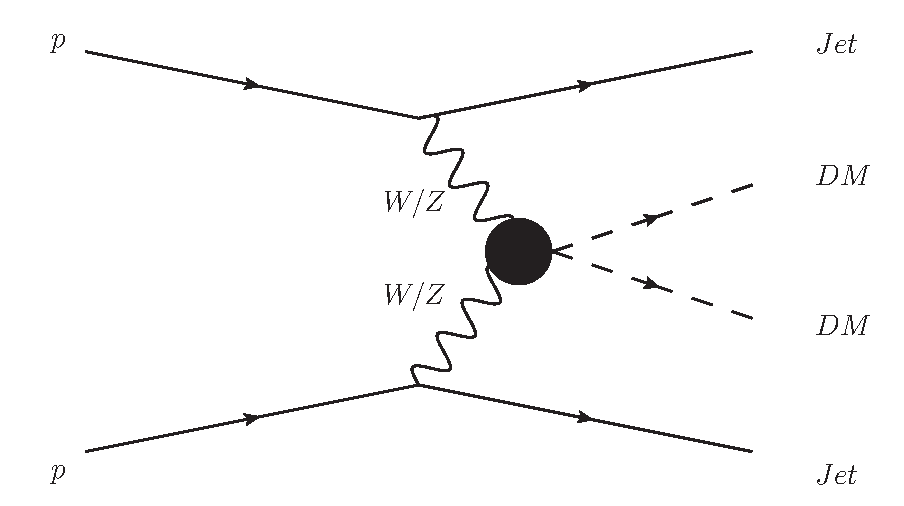
\includegraphics[width=1.\textwidth]{ppdmdmjj_feynman-eps-converted-to.pdf}
\label{DMFeynman}
\end{subfigure}
\begin{subfigure}{.35\textwidth}
  \centering
\includegraphics[width=1.\textwidth]{ppdmdmjj_feynman_z}
\label{DMFeynmanwithz}
\end{subfigure}
\begin{subfigure}{.30\textwidth}
  \centering
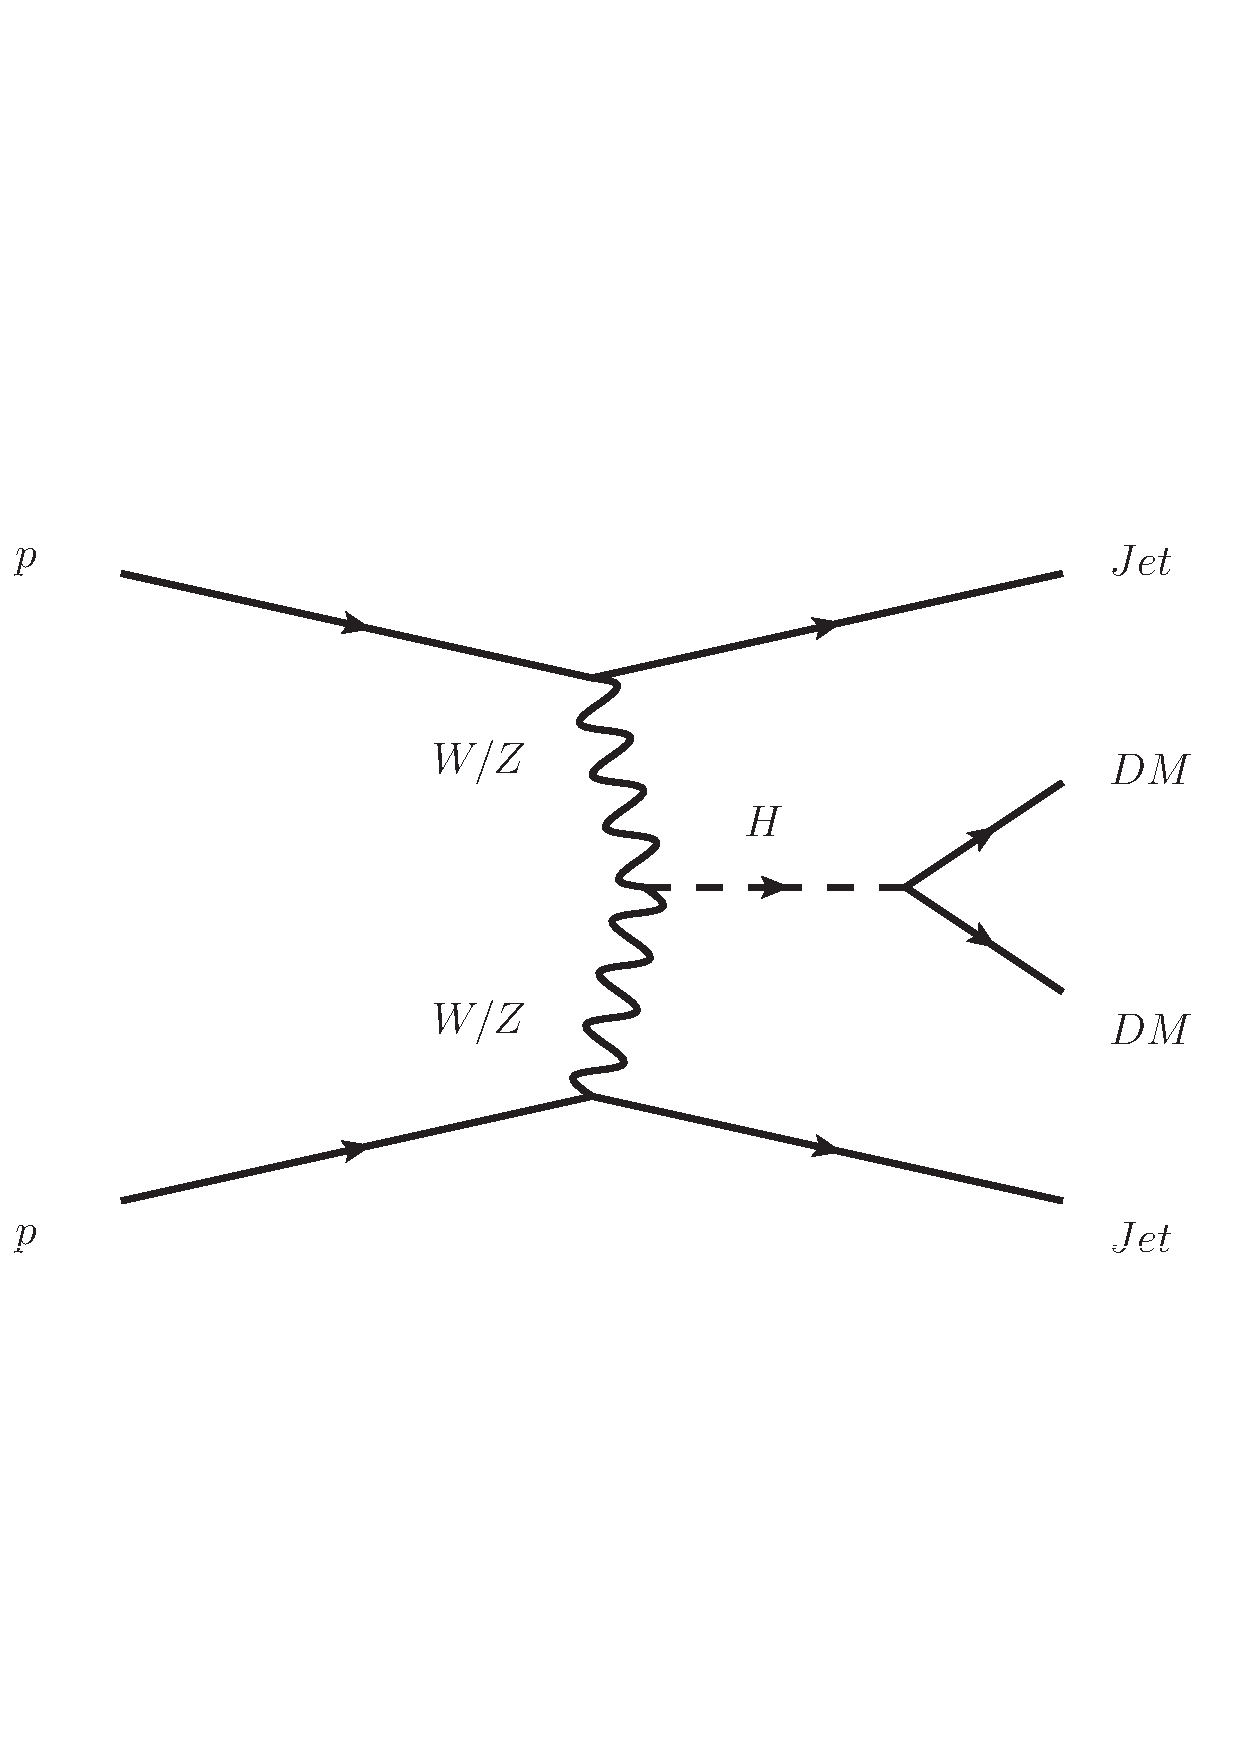
\includegraphics[width=1.\textwidth]{pphiggsdmdmjj}
\label{DMFeynmanwithHiggs}
\end{subfigure}
\label{VBFDM}
\end{figure}
\end{block}
\end{frame}

\begin{frame}
\frametitle{Planned Models}
Monojet Models:
\begin{itemize}
\item Plan to run any existing monojet models through our analysis and limit setting code.
\item Are there any suggestions any other Monojet MCs or simplified models that should be looked at? \newline
\end{itemize}
VBF Models:
\begin{itemize}
\item Again, plan to run over any existing MC models through our analysis and limit setting code.
\item Happy to run over simplified models for VBF, if they exist?
\begin{itemize}
\item Currently only aware of EFT implementation [PRD 88 116009 (2013)].
\item Using this EFT model to validate our analysis and limit setting framework, but will be straight forward to replace with any other model. 
\end{itemize}
\item Any other thoughts/models?
\end{itemize}
\end{frame}

\iffalse
\begin{frame}
\begin{itemize}
\item Will give an overview of what models of dark matter production this measurement is particularly sensitive to, what new sensitivity it brings both in terms of specific models and how this can be used for already existing models. \newline
\item Look at BSM interpretation of this analysis of VBF to dark matter using EFTs. \newline 
\item Specific strengths of this search for dark matter:
\begin{itemize}
\item Focus on general topologies/interactions: quark/gluon-DM interactions (monojet), electroweak boson - DM interactions (VBF)
\item Corrected dark matter observables for detector effects.
\item Will publish the data distributions, statistical and systematic uncertainties bin by bin, and any relevant correlation information (between two+ 1D distributions) to allow any theorist to compare their DM model predictions to our data in future without any bias.\newline
\end{itemize}
\item Using the measured ratio, limits can be se on a general model.
\end{itemize}
\end{frame}
\fi


\begin{frame}
\frametitle{Idea of this measurement}
\begin{itemize}
\item EFT models mentioned in the previous slide are only providing a benchmark, and any model will be comparable to our published data using our rivet analysis code after publication.
\item Difference from existing VBF and monojet searches:
\begin{itemize}
\item Measure corrected differential ratio as a function of various observables (Mjj, jet1pt, deltaphijj,)
\item Publish alongside paper:
\begin{itemize}
\item Cross section ratio in each bin 
\item Statistical and systematic correlations between bins
\item Rivet routine for post-publication model analysis
\end{itemize}
\end{itemize}
\item This analysis approach is not optimised for specific searches (like H$\rightarrow$invisible) so have tradeoff of reduced sensitivity to these specific models for improved sensitivity to other general production modes.
\item Next slides show details of DM in the EFT models.
\end{itemize}
\end{frame}

%\iffalse
%\begin{frame}
%\frametitle{Models being tested}
%\begin{block}{VBF DM models}
%\begin{itemize}
%\item Run over whatever MC models exist for VBF topologies used in the past:
%\begin{itemize}
%\item H $\rightarrow$ MET + jj
%\item Z $\rightarrow$ MET + jj
%\end{itemize}
%\item Can use simplified models if they exist $\rightarrow$ Only currently aware of general EFTs (But will process whatever is available).
%\item These EFTs are only providing a benchmark, and any model will be comparable to our published data using our rivet analysis code after publication.
%\end{itemize}
%\end{block}
%\begin{exampleblock}{$\geqslant$ 1 jet / Monojet models}
%\begin{itemize}
%\item Run over monojet DM searches to look at:
%\begin{itemize}
%\item Z $\rightarrow$ MET + j
%\item W $\rightarrow$ MET + j
%\end{itemize}
%\item Run our analysis over MC models: through a rivet routine and limit setting code and check sensitivity to these models. 
%\end{itemize}
%\end{exampleblock}
%\end{frame}
%\fi

\begin{frame}
\frametitle{MadGraph simulation using VBF EFT models}
MadGraph implemenation discussed in [PRD 88 116009 (2013)] 
\begin{table}[H]
\begin{center}
\scriptsize
 \begin{tabular}{ c | c  } 
 \hline \hline
 Name & Operator  \\ \hline \hline
 D5a & $\mathcal{L} = \frac{1}{\Lambda}\bar{\chi}\chi\bigg[\frac{Z_{\mu}Z^{\mu}}{2}+W_{\mu}^{+}W^{-\mu}\bigg]$  \\
 D5b & $\mathcal{L} = \frac{1}{\Lambda}\bar{\chi}\gamma^{5}\chi\bigg[\frac{Z_{\mu}Z^{\mu}}{2}+W_{\mu}^{+}W^{-\mu}\bigg]$  \\
 D5c & $\mathcal{L} = \frac{g}{2\cos{\theta_{W}}\Lambda}\bar{\chi}\sigma^{\mu\nu}\chi\bigg[\delta_{\mu}Z_{\nu}-\delta_{\nu}Z_{\mu}\bigg]$  \\
 D5d & $\mathcal{L} = \frac{g}{2\cos{\theta_{W}}\Lambda}\bar{\chi}\sigma^{\mu\nu}\chi\epsilon^{\mu\nu\sigma\rho}\bigg[\delta_{\rho}Z_{\sigma}-\delta_{\sigma}Z_{\rho}\bigg]$  \\
 D6a & $\mathcal{L} = \frac{g}{2\cos{\theta_{W}}\Lambda^{2}}\bar{\chi}\gamma^{\mu}\delta^{\nu}\chi\bigg[\delta_{\mu}Z_{\nu}-\delta_{\nu}Z_{\mu}\bigg]$  \\
 D6b & $\mathcal{L} = \frac{g}{2\cos{\theta_{W}}\Lambda^{2}}\bar{\chi}\gamma_{\mu}\delta_{\nu}\chi\epsilon^{\mu\nu\sigma\rho}\bigg[\delta_{\rho}Z_{\sigma}-\delta_{\sigma}Z_{\rho}\bigg]$  \\
 D7a & $\mathcal{L} = \frac{1}{\Lambda^{3}}\bar{\chi}\chi W^{i,\mu\nu}W_{\mu\nu}^{i}$  \\
 D7b & $\mathcal{L} = \frac{1}{\Lambda^{3}}\bar{\chi}\gamma^{5}\chi W^{i,\mu\nu}W_{\mu\nu}^{i}$  \\
 D7c & $\mathcal{L} = \frac{1}{\Lambda^{3}}\bar{\chi}\chi\epsilon^{\mu\nu\sigma\rho} W^{i,\mu\nu}W_{\rho\sigma}^{i}$  \\
 D7d & $\mathcal{L} = \frac{1}{\Lambda^{3}}\bar{\chi}\gamma^{5}\chi\epsilon^{\mu\nu\sigma\rho} W^{i,\mu\nu}W_{\rho\sigma}^{i}$  \\ \hline \hline
\end{tabular}
\end{center}
\end{table}
Original publication tested unitarity validity in VBF processes for mass-EFT scale probed in this analysis.
\end{frame}


\begin{frame}
\frametitle{MadGraph simulation using EFT models}
\begin{itemize}
\item Currently only generating exclusively two jets ($\chi\bar{\chi}$jj), but are in the process of interfacing these to a parton shower, so results very preliminary.
\begin{itemize}
\item Also generating other minor contributing processes: ($\chi\bar{\chi}l\nu$, $\chi\bar{\chi}ll$, $\chi\bar{\chi}ll$jj) \newline
\end{itemize}
\end{itemize}
\begin{columns}
\begin{column}{.32\textwidth}
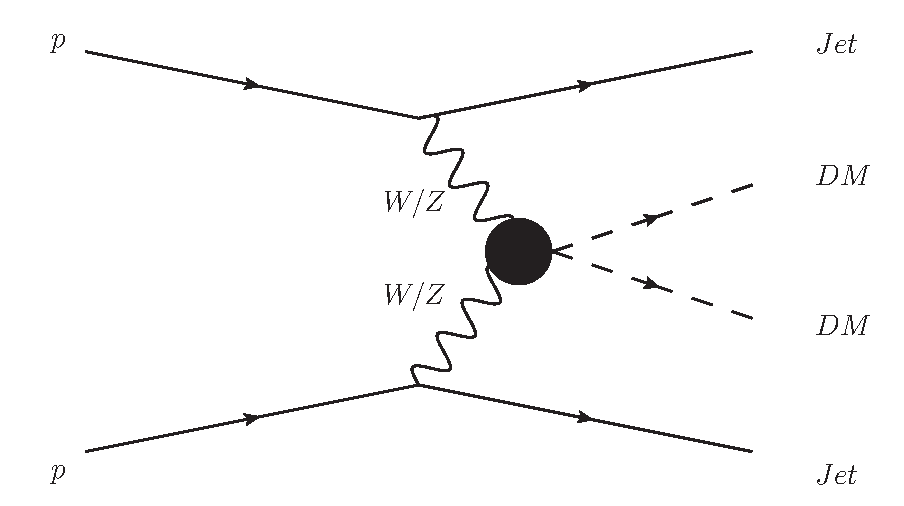
\includegraphics[width=1.\textwidth]{ppdmdmjj_feynman-eps-converted-to.pdf}
\newline
\end{column}
\begin{column}{.35\textwidth}
\includegraphics[width=1.\textwidth]{ppdmdmjj_feynman_z}
\newline
\end{column}
\begin{column}{.30\textwidth}
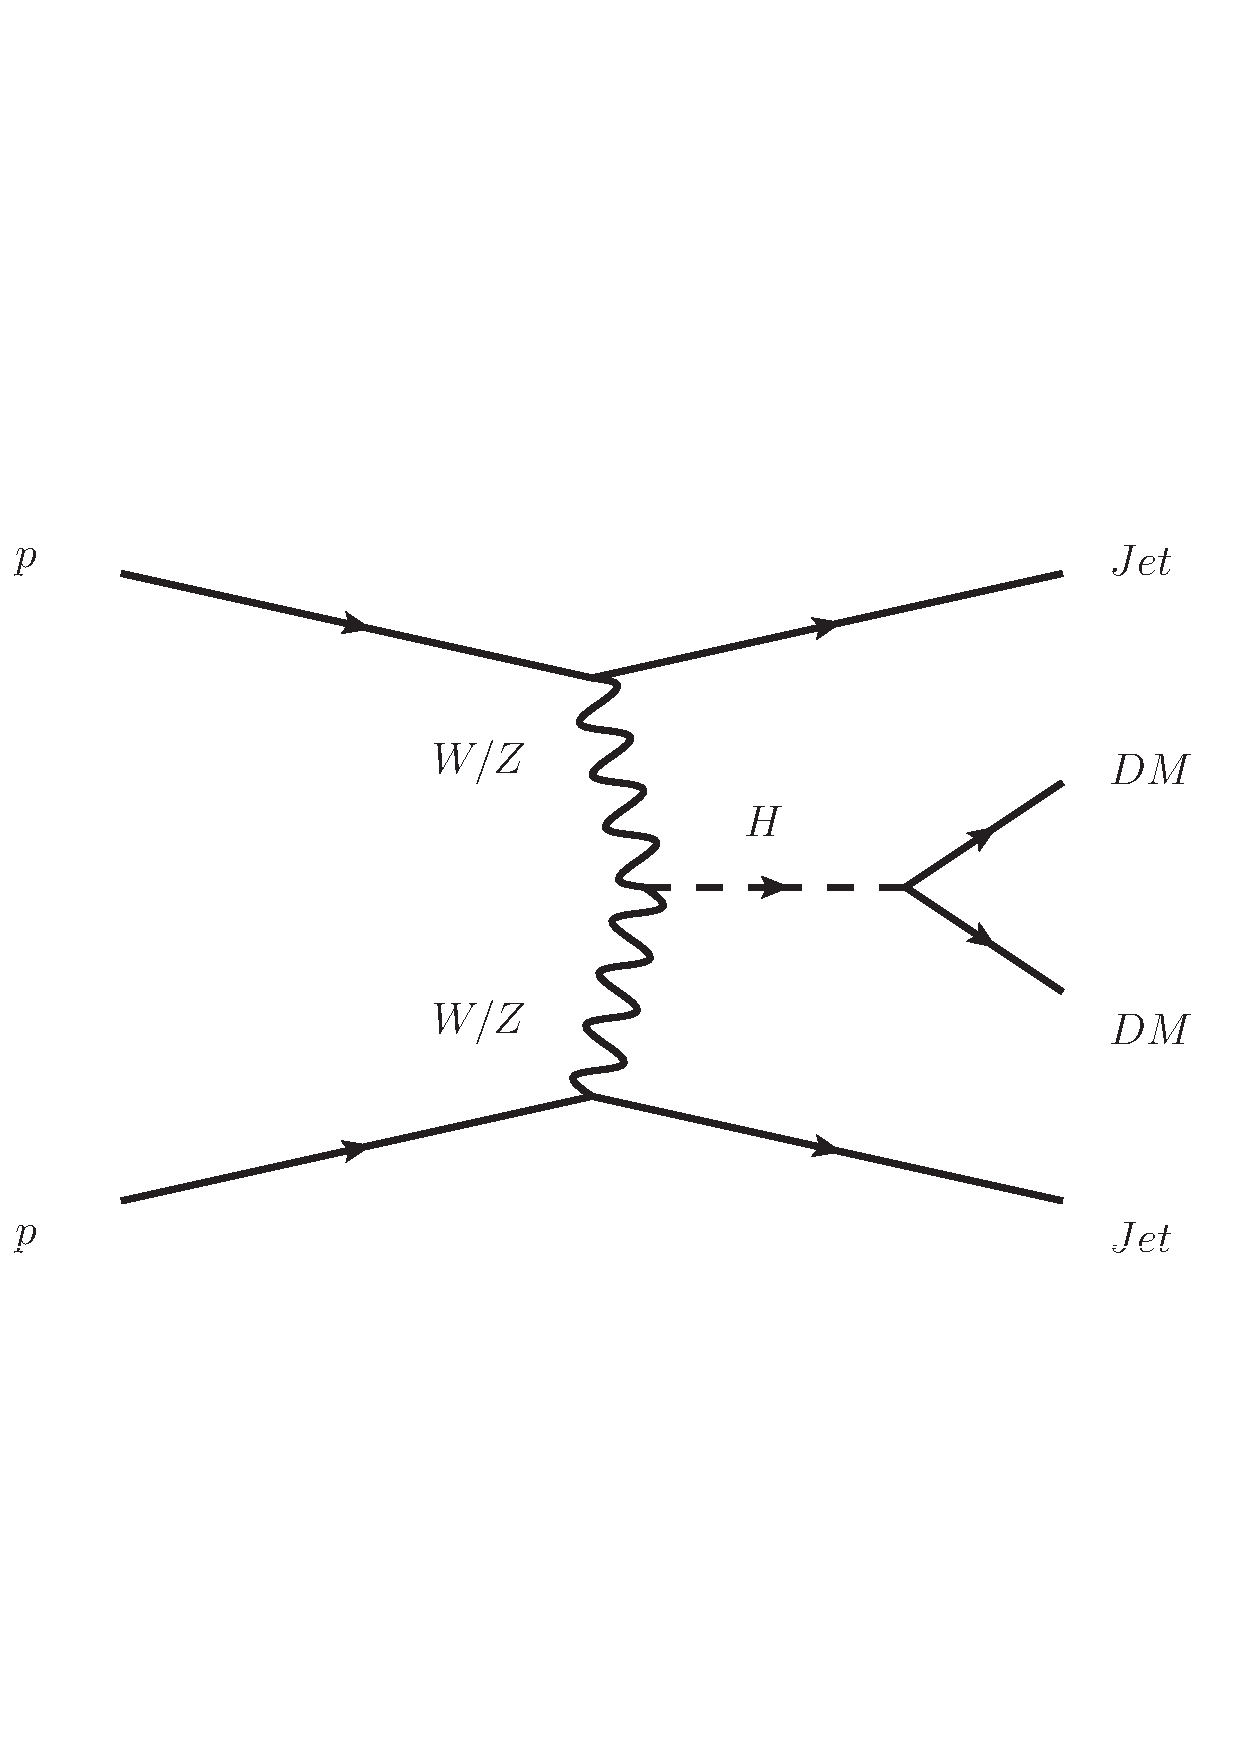
\includegraphics[width=1.\textwidth]{pphiggsdmdmjj}
\newline
\end{column}
\end{columns}

\end{frame}


\begin{frame}
\frametitle{EFT scale constraints from SM measurements}
\begin{itemize}
\item \small{The different dimensions that have the higher EFT scale constraints result in some dimensions with vastly reduced rates due to the Z invisible width.}

\center{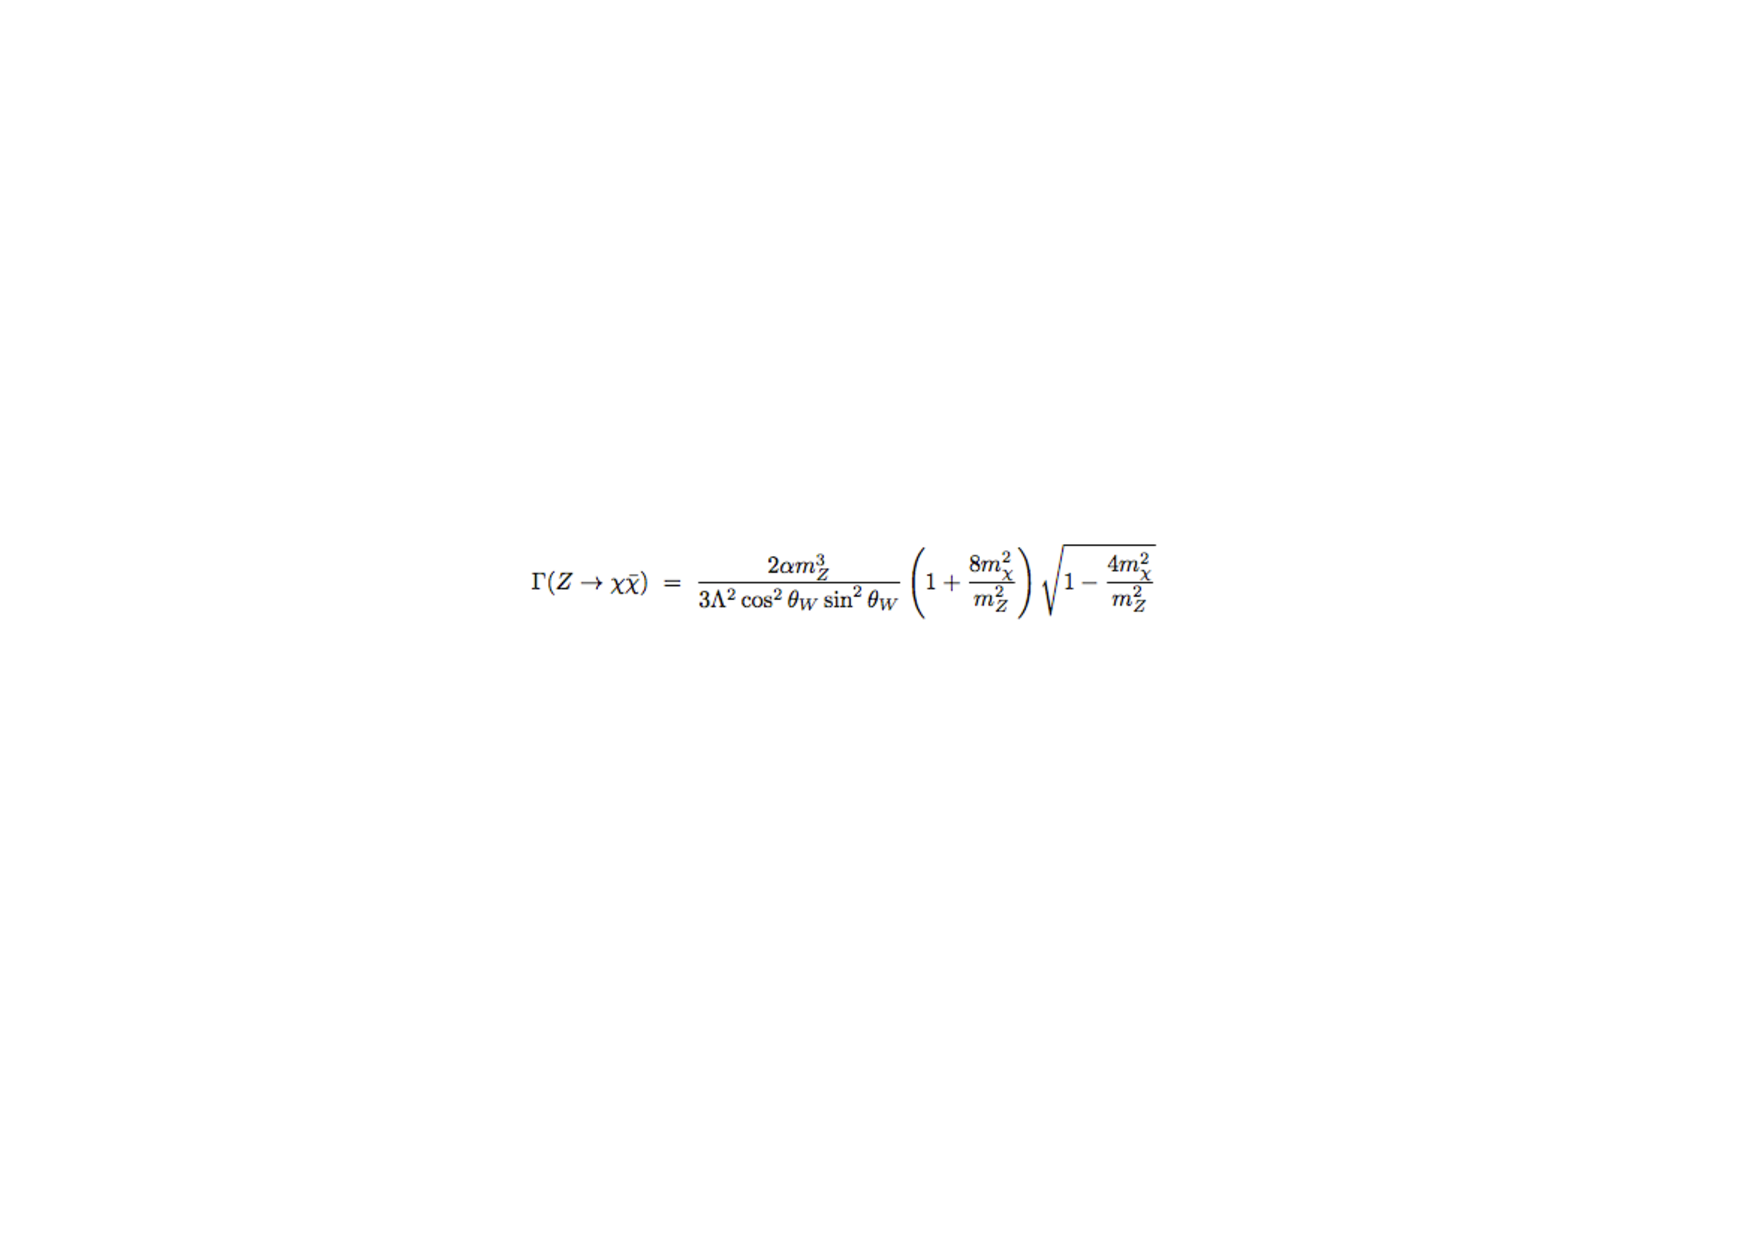
\includegraphics[width=0.5\linewidth]{D5a_Rate_Equation}}
\end{itemize}
\begin{table}[H]
\begin{center}
\scriptsize
 \begin{tabular}{ c | c | c } 
 \hline \hline
 Name & Operator & Minimum EFT Scale (GeV) \\ \hline \hline
 D5a & $\mathcal{L} = \frac{1}{\Lambda}\bar{\chi}\chi\bigg[\frac{Z_{\mu}Z^{\mu}}{2}+W_{\mu}^{+}W^{-\mu}\bigg]$ & 100 \\
 D5b & $\mathcal{L} = \frac{1}{\Lambda}\bar{\chi}\gamma^{5}\chi\bigg[\frac{Z_{\mu}Z^{\mu}}{2}+W_{\mu}^{+}W^{-\mu}\bigg]$ & 100 \\
 D5c & $\mathcal{L} = \frac{g}{2\cos{\theta_{W}}\Lambda}\bar{\chi}\sigma^{\mu\nu}\chi\bigg[\delta_{\mu}Z_{\nu}-\delta_{\nu}Z_{\mu}\bigg]$ & 3300 \\
 D5d & $\mathcal{L} = \frac{g}{2\cos{\theta_{W}}\Lambda}\bar{\chi}\sigma^{\mu\nu}\chi\epsilon^{\mu\nu\sigma\rho}\bigg[\delta_{\rho}Z_{\sigma}-\delta_{\sigma}Z_{\rho}\bigg]$ & 6600 \\
 D6a & $\mathcal{L} = \frac{g}{2\cos{\theta_{W}}\Lambda^{2}}\bar{\chi}\gamma^{\mu}\delta^{\nu}\chi\bigg[\delta_{\mu}Z_{\nu}-\delta_{\nu}Z_{\mu}\bigg]$ & 230 \\
 D6b & $\mathcal{L} = \frac{g}{2\cos{\theta_{W}}\Lambda^{2}}\bar{\chi}\gamma_{\mu}\delta_{\nu}\chi\epsilon^{\mu\nu\sigma\rho}\bigg[\delta_{\rho}Z_{\sigma}-\delta_{\sigma}Z_{\rho}\bigg]$ & 330 \\
 D7a & $\mathcal{L} = \frac{1}{\Lambda^{3}}\bar{\chi}\chi W^{i,\mu\nu}W_{\mu\nu}^{i}$ & 100 \\
 D7b & $\mathcal{L} = \frac{1}{\Lambda^{3}}\bar{\chi}\gamma^{5}\chi W^{i,\mu\nu}W_{\mu\nu}^{i}$ & 100 \\
 D7c & $\mathcal{L} = \frac{1}{\Lambda^{3}}\bar{\chi}\chi\epsilon^{\mu\nu\sigma\rho} W^{i,\mu\nu}W_{\rho\sigma}^{i}$ & 100 \\
 D7d & $\mathcal{L} = \frac{1}{\Lambda^{3}}\bar{\chi}\gamma^{5}\chi\epsilon^{\mu\nu\sigma\rho} W^{i,\mu\nu}W_{\rho\sigma}^{i}$ & 100 \\ \hline \hline
\end{tabular}
\end{center}
\end{table}
\end{frame}

\begin{frame}
\frametitle{Model Kinematics: Distinguishing DM operators}
\begin{itemize}
\item Plots show unit normalised DM distributions for DM mass = 100GeV
\end{itemize}
\begin{columns}
\begin{column}{.33\textwidth}
\includegraphics[width=.8\textwidth]{Mass100/Normalised/NOBKG/Mass100_Mjj_PS_VBFDM.pdf}
\newline
\includegraphics[width=.8\textwidth]{Mass100/Normalised/NOBKG/Mass100_DeltaEta_PS_VBFDM.pdf}
\end{column}
\begin{column}{.33\textwidth}
\includegraphics[width=.8\textwidth]{Mass100/Normalised/NOBKG/Mass100_Etmiss_PS_VBFDM.pdf}\newline
\includegraphics[width=.8\textwidth]{Mass100/Normalised/NOBKG/Mass100_Jet1Pt_PS_VBFDM.pdf}
\end{column}
\begin{column}{.33\textwidth}
\includegraphics[width=.8\textwidth]{Mass100/Normalised/NOBKG/Mass100_DeltaPhi_PS_VBFDM.pdf} \newline \newline \newline
Discrimination between models varies with observable studied: Motivation to measure multiple observables.
\end{column}
\end{columns}
\end{frame}

\begin{frame}
\frametitle{Model Kinematics: Distinguishing DM Mass}
\begin{itemize}
\item Plots show unit normalised DM distributions for leading jet $p_T$ and $\Delta\phi$
\end{itemize}
\begin{columns}
\begin{column}{.1\textwidth}
\newline
1GeV \newline \newline \newline \newline \newline \newline \newline \newline
1TeV \vspace{2cm}
\end{column}
\begin{column}{.3\textwidth}
\center{$\Delta\Phi$}
\includegraphics[width=.9\textwidth]{Mass1/Normalised/NOBKG/Mass1_DeltaPhi_PS_VBFDM.pdf}
\newline
\includegraphics[width=.9\textwidth]{Mass1000/Normalised/NOBKG/Mass1000_DeltaPhi_PS_VBFDM.pdf}
\end{column}
\begin{column}{.3\textwidth}
\center{Jet 1 pT}
\includegraphics[width=.9\textwidth]{Mass1/Normalised/NOBKG/Mass1_Jet1Pt_PS_VBFDM.pdf}\newline
\includegraphics[width=.9\textwidth]{Mass1000/Normalised/NOBKG/Mass1000_Jet1Pt_PS_VBFDM.pdf}
\end{column}
\begin{column}{.3\textwidth}
\begin{itemize}
\item These observables are also sensitive to the mass of the dark matter.
\item Can also exploit correlations between distributions for increased sensitivity.
\end{itemize}
\end{column}
\end{columns}
\end{frame}

\begin{frame}
\frametitle{From DM kinematics to Ratio}
\begin{itemize}
\item Previous slides show DM production rate kinematics
\item We measure the ratio \textcolor{purple}{$\frac{\sigma(\textrm{Z}\rightarrow\nu\bar{\nu}+\textrm{j(j)})}{\sigma(\textrm{Z}\rightarrow l^{+}l^{-}+\textrm{j(j)})}$} in data, so DM presence causes modification to shape and normalisation of this ratio
\item SM expectation is flat value of approx. 6 $\rightarrow$, modified in measured data due to acceptance differences in numerator and denominator \newline
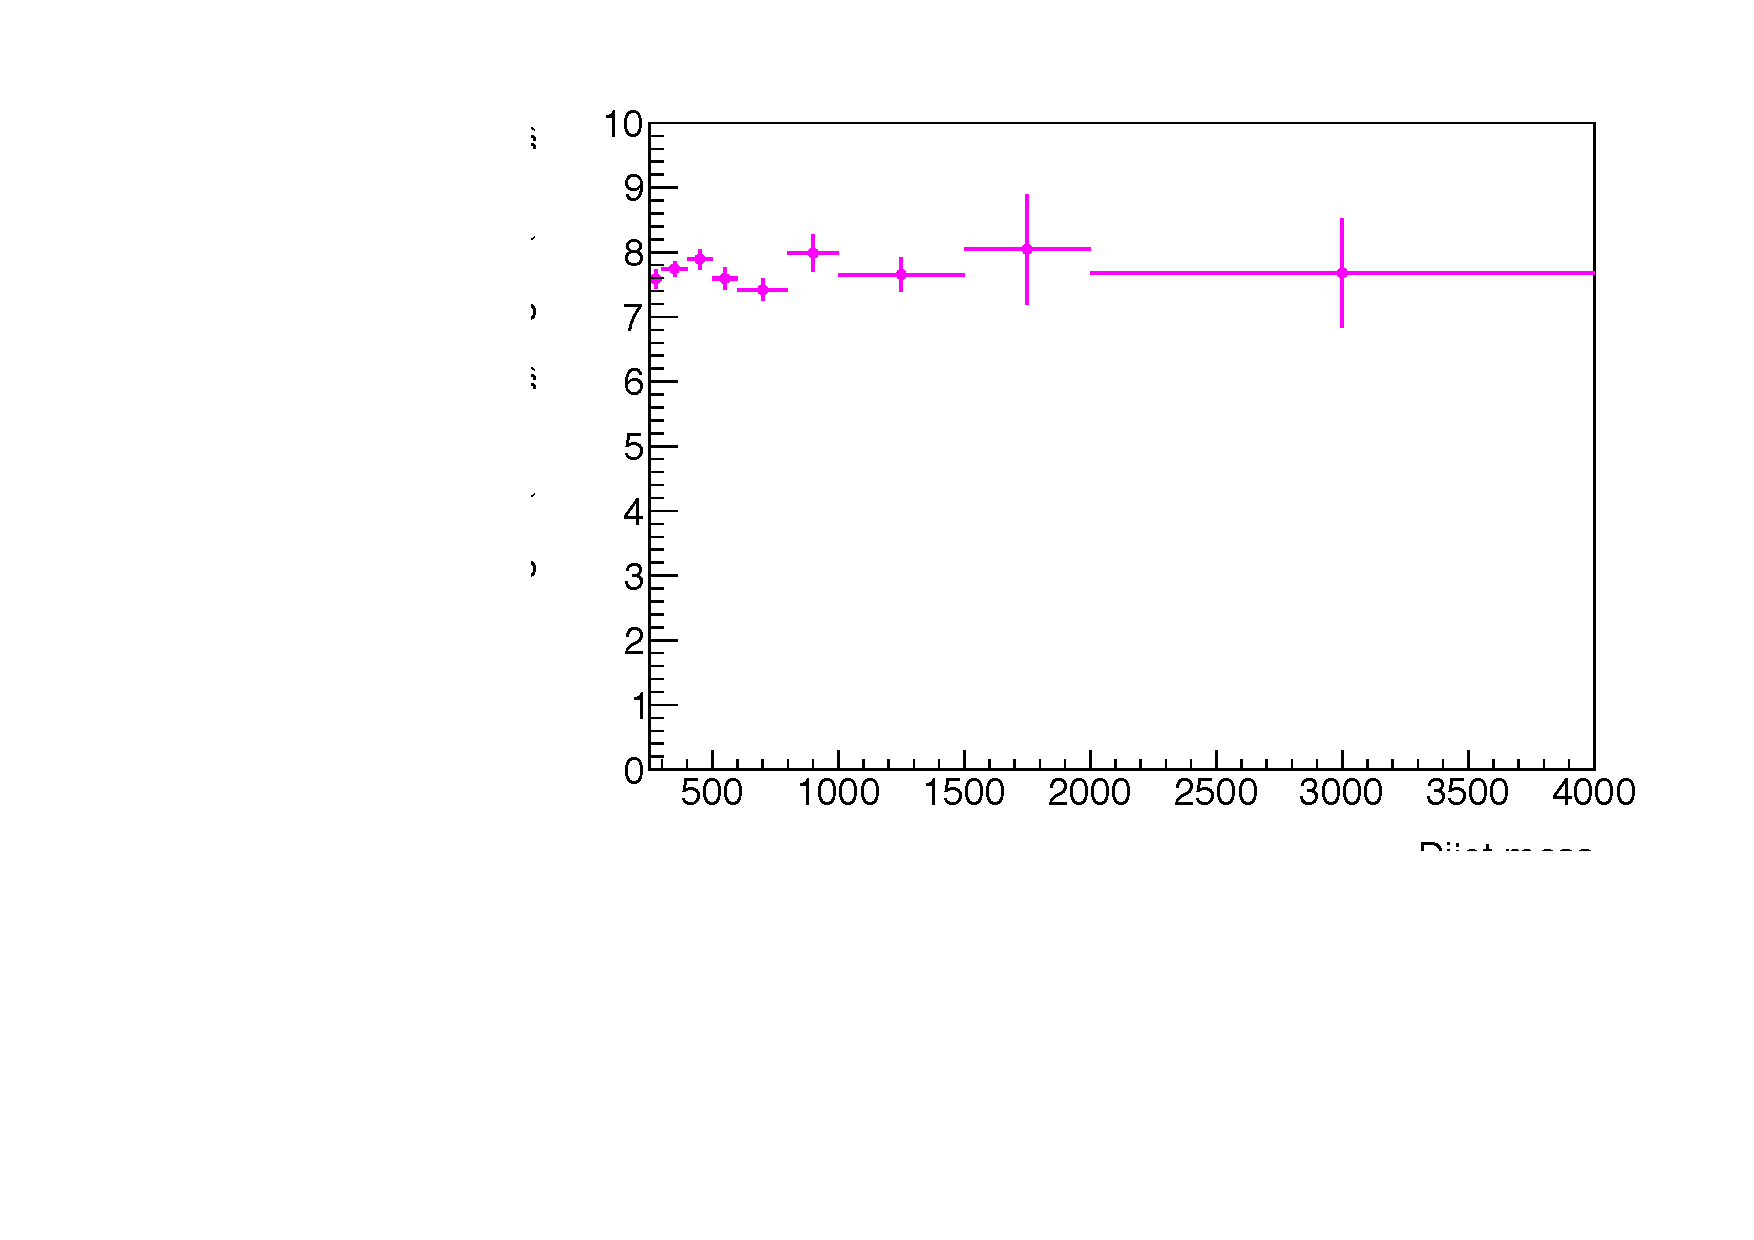
\includegraphics[width=.4\textwidth]{c1.pdf}
\item Next slides will show modification of this ratio with DM present
\end{itemize}
\end{frame}

\begin{frame}
\frametitle{Example of ratio modification with DM}
\center Effective Operator D5a : $\Delta\eta$ : $\Lambda_{Min}$ = 100GeV : 2\% statistical uncertainty : P-value of chi2 stat. test.
\center
\includegraphics[width=10cm]{/D5a/Absolute/0.02/Stats_D5a_DeltaEta_002_PS_VBFDM.pdf}
\begin{itemize}
\item Ratio plot shows $\frac{\sigma((Z\rightarrow\nu\nu)jj)+\sigma((Z\rightarrow DM DM)jj)}{\sigma((Z\rightarrow\mu^{+}\mu^{-})jj)}_{(EWK+QCD)}$
\item $p$-value from a $\chi^{2}$-test comparing the DM model to the SM background ratio of $\frac{\sigma((Z\rightarrow\nu\nu)jj)}{\sigma((Z\rightarrow\mu^{+}\mu^{-})jj)}$, for a range of DM masses and EFT scales.
\end{itemize}
\end{frame}

\begin{frame}
\frametitle{Example of ratio modification with DM}
\center{Effective Operator D5a : Mjj : $\Lambda_{Min}$ = 100GeV : 2\% statistical uncertainty : P-value of chi2 stat. test.}
\center
\includegraphics[width=10cm]{/D5a/Absolute/0.02/Stats_D5a_Mjj_002_PS_VBFDM.pdf}
\end{frame}

\begin{frame}
\frametitle{Example of ratio modification with DM}
\center{Effective Operator D5b : Mjj : $\Lambda_{Min}$ = 100GeV : 2\% statistical uncertainty : P-value of chi2 stat. test.}
\center
\includegraphics[width=10cm]{/D5b/Absolute/0.02/Stats_D5b_Mjj_002_PS_VBFDM.pdf}
\begin{itemize}
\item This is currently a work in progress as we are validating the implementation of the models. PS and CJV also not yet present.
\end{itemize}
\end{frame}


\iffalse
\begin{frame}
\frametitle{Example of ratio modification with DM}
\center{Effective Operator D5a : Mjj : $\Lambda_{Min}$ = 100GeV : $\sqrt{N}$ statistical uncertainty Luminosity of 3 fb$^{-1}$ : P-value of chi2 stat. test.}
\center
\includegraphics[width=10cm]{/D5a/Absolute/Lumi2015/Stats_D5a_Mjj_Lumi2015_PS_VBFDM.pdf}
\begin{itemize}
\item Sensitivity with 2015 Data of Luminosity 3 fb$^{-1}$.
\end{itemize}
\end{frame}

\begin{frame}
\frametitle{Example of ratio modification with DM}
\center{Effective Operator D5a : Mjj : $\Lambda_{Min}$ = 100GeV : $\sqrt{N}$ statistical uncertainty Luminosity of 30 fb$^{-1}$ : P-value of chi2 stat. test.}
\center
\includegraphics[width=10cm]{/D5a/Absolute/Lumi2016/Stats_D5a_Mjj_Lumi2016_PS_VBFDM.pdf}
\begin{itemize}
\item Sensitivity with 2016 Data of Luminosity 30 fb$^{-1}$.
\end{itemize}
\end{frame}
\fi

\begin{frame}
\frametitle{Summary and To Do}
\begin{itemize}
\item Differential measurement of $\frac{\sigma\textrm{(MET+j(j))}}{\sigma(\textrm{Z}\rightarrow l^{+}l^{-}+\textrm{j(j)})}$ sensitive to both quark/gluon and electroweak boson couplings to DM
\item Set up framework to test presence of DM models against SM expectation in variety of fiducial regions and for various observables
\item Currently running on VBF EFT model as a benchmark, plan to now extend to process existing Monojet/VBF DM signal MCs
\begin{itemize}
\item Simplified models for VBF? Who to contact?
\end{itemize}
\item Plan to publish Rivet routine with ratios and correlation information so new models can be easily compared to data also after publication
\item Next steps:
\begin{itemize}
\item Continue validation of models and analysis framework
\item Interface parton showering to Madgraph EFT implementation
\item Process existing Monojet/VBF MCs (and any other new models?)
\item Quantify sensitivity gains from correlations between differential ratios
\end{itemize}
\end{itemize}
\end{frame}


\end{document} 
